%Practicum LATEX UiE 2023

%Tipo de documento

\documentclass[12pt]{article}
%\documentclass{book}
%\documentclass{report}

%Paquete de Margenes
\usepackage[left= 2.5cm, right= 2.5cm, top= 2cm, bottom= 2cm]{geometry}

%Paquete Lenguaje
\usepackage[spanish]{babel}  %Es posible que se necesiten los pakages imputend y fontend

%Paquete Imagenes
\usepackage{graphicx}

%Paquetes Matematicas
\usepackage{amsmath, amsthm, amssymb, amsfonts}

%Paquete Hipervínculos
\usepackage{hyperref}

%Manual de paquetes en CTAN

%Documento

\title{\Huge Prácticum \Latex}
\author{\Large Manuel Mateo Delgado}
\date{01/03/2023}

\begin{document}

    \maketitle %Genera Portada


    \clearpage %Cambia de pagina

    \tableofcontents %Creamos Index

    \clearpage

    \section{Pruebas con equaciones}

        Este es un \textbf{documento} de prueba de instalacion del compilador de comandos de \textit{\Latex}. \smalllskip

        Veamos como insertar caracteres matemáticos dentro del texto y en formato ecuación. \smallskip 
        %Se puede utiizar \vspace{l} y \hspace{l}

        En primer lugar, insertamos la ecuación $x^2-1=0$. Una alternativa es utlilizar el entorno \textit{equation}, por ejemplo:

        \subsection{Ecuación Límite}
        
            \begin{equation}\label{LimInf}

                \lim_{n\to\infty}\left(1+ \frac{1}{n}\right)^n
                %Utilizamos \left y \right para ajustar el parentesis a lo de dentro de la equación
            \end{equation}

        \subsection{Ecuación Integral}  

            \begin{equation}\label{TFC} %Etiquetamos una función

                F(x) = \int_a^xf(t)dt %No se ponen $ en el entorno equation

            \end{equation}
            %Si queremos eliminar el [nº identificador] se escribe \begin{equation*} \end{equation*}

        La expresión \eqref{TFC} aparece en el Teorema Fundamental del Cálculo.
        La equación \eqref{LimInf} pretenece a un límite.

        Podemos utilizar el alfabeto griego:
        $\alpha$, $\beta$, $\sigma$, $\gamma$ \dots
        \exists un $n\in\mathbb{n}$ \backslash 

        \subsection{Prueba con raíces}

            \begin{equation}
                \sqrt[3]{\frac{1}{n^2-1}} < \varepsilon
            \end{equation}

    \section{Prueba con imágenes}

        %Introducimos una gráfica
        \begin{figure}[ht]\label{Grafica1}

            \centering %Centrar
            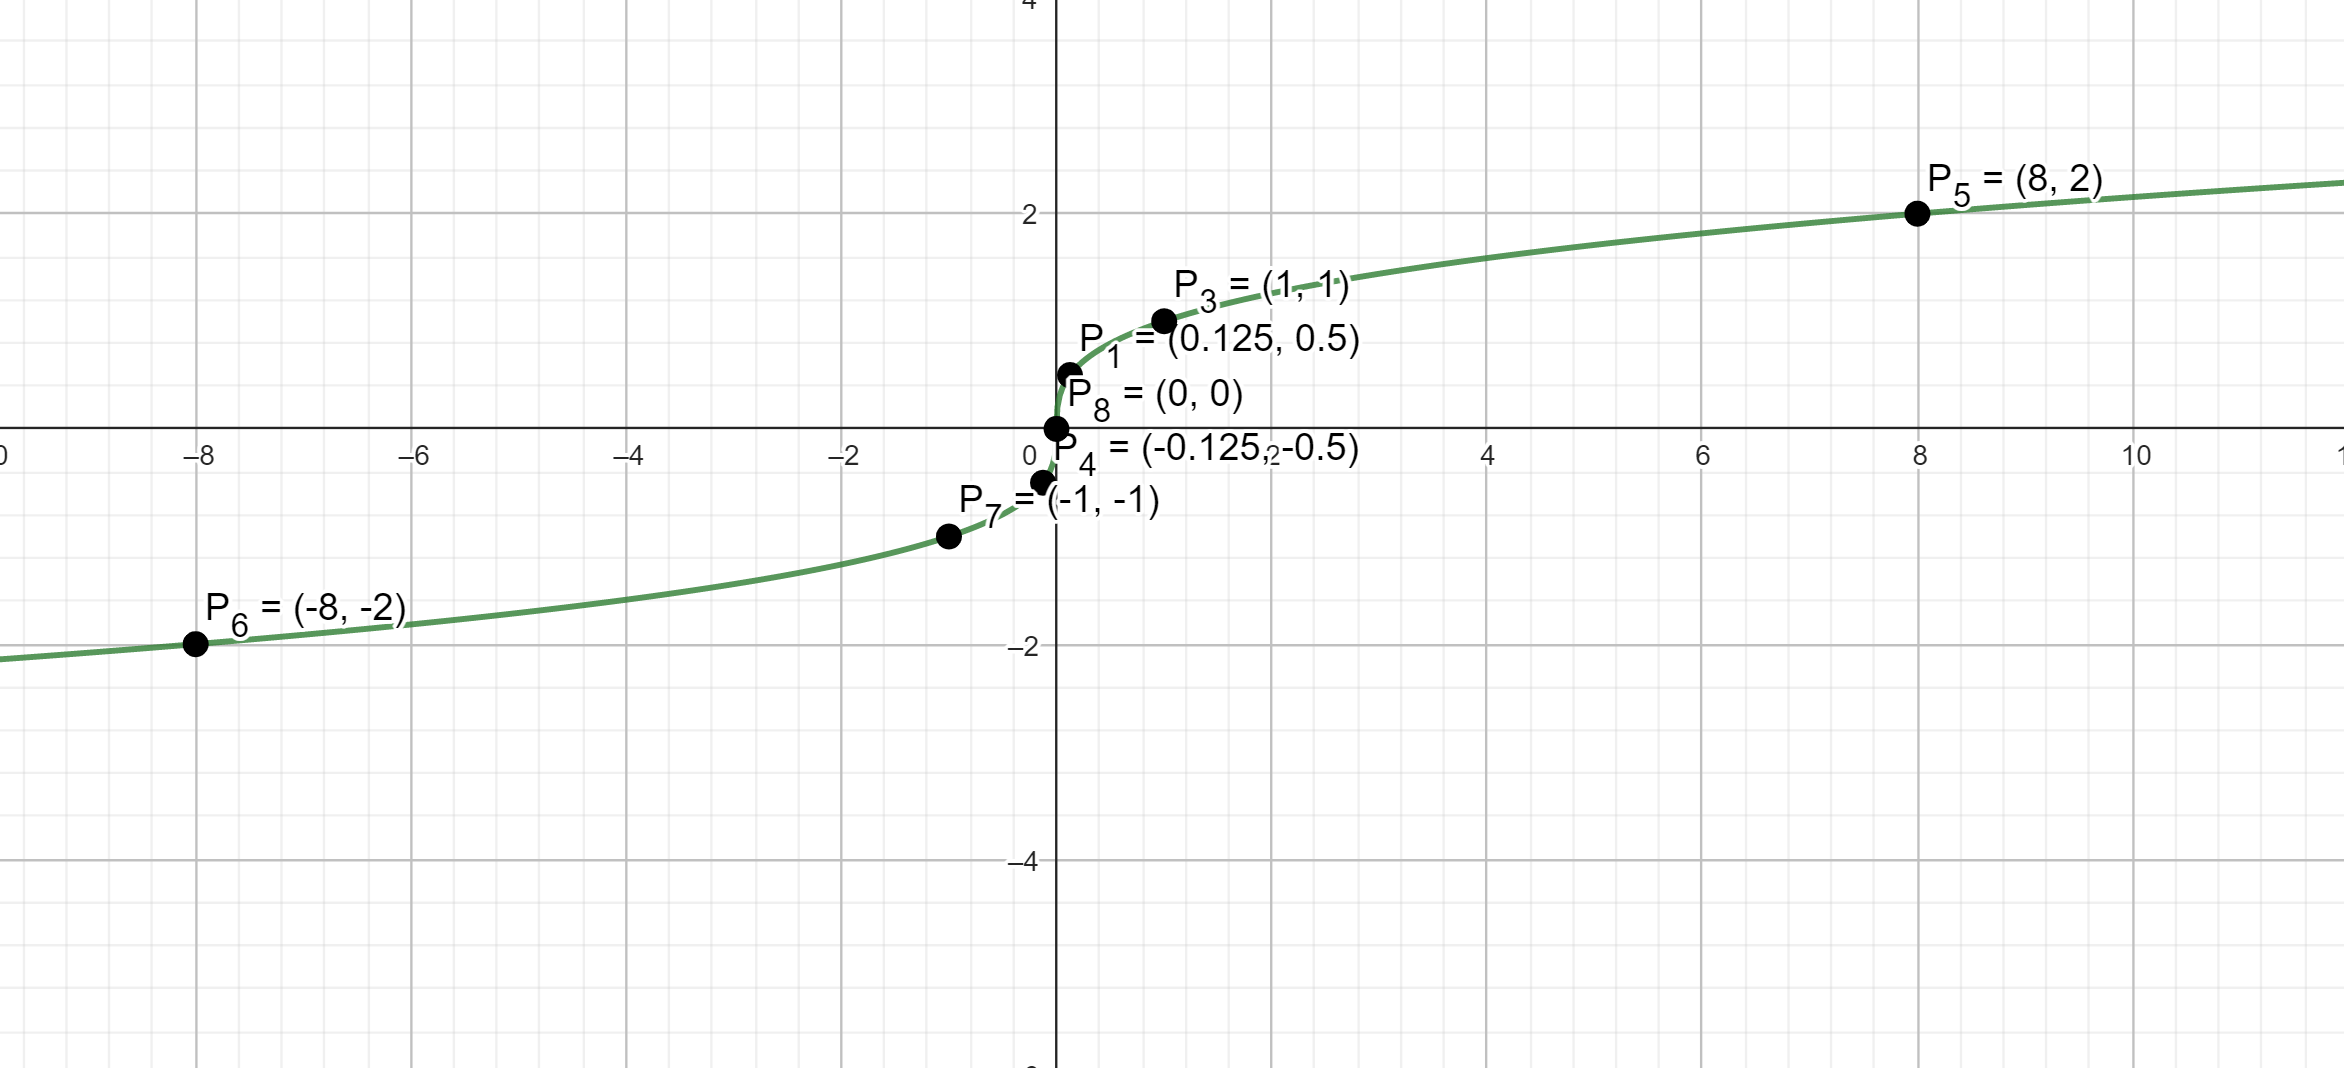
\includegraphics[width=10cm]{graficaboletin.png} %Archivo a introducir
            \caption[short]{title} %Pie de imagen/ título

        \end{figure}

        En la figura \ref{Grafica1} podemos ver la captura de pantalla.

        Podemos citar una referencia con el comando \cite{Grillo}.

    \section{bibliography}

        \begin{thebibliography}{99}

            \bibitem{Grillo} P. Grillo. \textit{Pinocho y sus aventuras}. Editorial aaaaa. Lugar bbbbb. 1900.
            \bibitem{OverLeaf}\href{https://www.overleaf.com}{Página web de OverLeaf}
        
        \end{thebibliography}

    \section{Listas}
        
        \begin{itemize}

            \item[a)] Fruta
            \item[b)] Leche
            \item[c)] Huevos
            \item[d)] Aguacate
            
        \end{itemize}

        \begin{enumerate}
            
            \item Cálculo
            \item Metodología
            \item Estructura de Datos
            
        \end{enumerate}

\end{document}